% =====================================================================
%  Proyecto Final Integrador - Análisis de Algoritmos (SIST0175)
%  Grupo 6 - Informe técnico final (sesión 4): componentes C1 a C6
%  Compila con XeLaTeX o con pdfLaTeX (en Overleaf: Menu > Compiler).
% =====================================================================
\documentclass[11pt,letterpaper]{article}
\usepackage{iftex}
\ifXeTeX
  \usepackage{fontspec}
  \usepackage{polyglossia}
  \setmainlanguage{spanish}
  \gappto\captionsspanish{\renewcommand{\tablename}{Tabla}\renewcommand{\listtablename}{Índice de tablas}}
\else
  \usepackage[utf8]{inputenc}
  \usepackage[T1]{fontenc}
  \usepackage{lmodern}
  \usepackage[spanish,es-noshorthands,es-nodecimaldot,es-tabla]{babel}
\fi
\usepackage[margin=2.1cm,top=2.2cm,bottom=2.2cm]{geometry}
\usepackage{amsmath,amssymb,amsthm,mathtools}
\usepackage{graphicx,float,booktabs,array,tabularx,multirow}
\usepackage[table]{xcolor}
\usepackage{caption,subcaption}
\usepackage{algorithm}
\usepackage[noend]{algpseudocode}
\usepackage{tikz}
\usetikzlibrary{arrows.meta,positioning,fit,backgrounds,calc}
\usepackage{enumitem}
\usepackage{fancyhdr}
\usepackage{listings}
\definecolor{codfondo}{HTML}{F7F9FB}
\definecolor{codcoment}{HTML}{3B7D4F}
\definecolor{codcadena}{HTML}{A3452C}
\definecolor{codclave}{HTML}{1F5FA0}
\lstset{
  language=Python, basicstyle=\ttfamily\scriptsize, columns=fullflexible, keepspaces=true,
  backgroundcolor=\color{codfondo}, frame=single, rulecolor=\color{gris!40},
  numbers=left, numberstyle=\tiny\color{gris}, numbersep=6pt, xleftmargin=1.6em,
  breaklines=true, breakatwhitespace=false, postbreak=\mbox{\textcolor{gris}{$\hookrightarrow$}\space},
  keywordstyle=\color{codclave}\bfseries, commentstyle=\color{codcoment}\itshape,
  stringstyle=\color{codcadena}, showstringspaces=false, tabsize=4, upquote=true,
  extendedchars=true,
  literate={á}{{\'a}}1 {é}{{\'e}}1 {í}{{\'i}}1 {ó}{{\'o}}1 {ú}{{\'u}}1 {ñ}{{\~n}}1
           {Á}{{\'A}}1 {É}{{\'E}}1 {Í}{{\'I}}1 {Ó}{{\'O}}1 {Ú}{{\'U}}1 {Ñ}{{\~N}}1
           {¿}{{?`}}1 {¡}{{!`}}1 {²}{{\textsuperscript{2}}}1 {³}{{\textsuperscript{3}}}1
           {ĉ}{{$\hat{c}$}}1 {Θ}{{$\Theta$}}1 {Σ}{{$\Sigma$}}1 {φ}{{$\varphi$}}1
           {⌈}{{$\lceil$}}1 {⌉}{{$\rceil$}}1 {≤}{{$\le$}}1 {≥}{{$\ge$}}1 {→}{{$\to$}}1
}
\lstdefinestyle{salida}{language={}, numbers=none, xleftmargin=0pt, keywordstyle={}, commentstyle={}, stringstyle={}}
\newcommand{\codigo}[2]{\par\smallskip\noindent{\small\bfseries\texttt{\detokenize{#1}}}\enspace{\small\color{gris}#2}\lstinputlisting{codigo/#1}}
\usepackage[hidelinks]{hyperref}

\definecolor{azul}{HTML}{2A6FB0}
\definecolor{gris}{HTML}{5F6B76}
\definecolor{fondo}{HTML}{EEF3F8}
\captionsetup{font=small,labelfont=bf}
\setlist{itemsep=2pt,topsep=3pt}
\setlength{\parskip}{4pt}
\setlength{\parindent}{0pt}
\emergencystretch=3em
\tolerance=2000

\pagestyle{fancy}
\fancyhf{}
\lhead{\small\color{gris}Análisis de Algoritmos (SIST0175) -- Grupo 6}
\rhead{\small\color{gris}Informe técnico final}
\cfoot{\small\thepage}
\renewcommand{\headrulewidth}{0.3pt}

% Pseudocódigo en español
\floatname{algorithm}{Algoritmo}
\algrenewcommand\algorithmicwhile{\textbf{mientras}}
\algrenewcommand\algorithmicdo{\textbf{hacer}}
\algrenewcommand\algorithmicfor{\textbf{para}}
\algrenewcommand\algorithmicif{\textbf{si}}
\algrenewcommand\algorithmicthen{\textbf{entonces}}
\algrenewcommand\algorithmicelse{\textbf{si no}}
\algrenewcommand\algorithmicreturn{\textbf{devolver}}
\algrenewcommand\algorithmicfunction{\textbf{función}}
\algrenewcommand\algorithmicrequire{\textbf{Entrada:}}
\algrenewcommand\algorithmicensure{\textbf{Salida:}}
\algrenewcommand{\algorithmiccomment}[1]{\hfill{\color{gris}\(\triangleright\) #1}}

\theoremstyle{plain}
\newtheorem{teorema}{Teorema}
\newtheorem{lema}{Lema}
\theoremstyle{definition}
\newtheorem{definicion}{Definición}
\newcommand{\Th}{\Theta}
\newcommand{\Om}{\Omega}
\newcommand{\cajah}[1]{\par\smallskip\colorbox{fondo}{\parbox{\dimexpr\linewidth-2\fboxsep}{\small #1}}\par\smallskip}

% Generado por informe/generar_valores.py a partir de resultados/*.json. No editar a mano.
\newcommand{\cUnoPendUni}{1{,}22}
\newcommand{\cUnoPendAgr}{1{,}22}
\newcommand{\cUnoPendVer}{1{,}24}
\newcommand{\cUnoPendFB}{1{,}89}
\newcommand{\cUnoPendTeo}{1{,}11}
\newcommand{\cUnoBajoMin}{1{,}13}
\newcommand{\cUnoBajoMax}{1{,}16}
\newcommand{\cUnoAltoMin}{1{,}28}
\newcommand{\cUnoAltoMax}{1{,}30}
\newcommand{\cUnoPendComb}{1{,}11}
\newcommand{\cUnoPendDist}{1{,}01}
\newcommand{\cUnoMaxVecinos}{2}
\newcommand{\cUnoSpeedup}{47{,}0}
\newcommand{\cUnoCruce}{64}
\newcommand{\cUnoCombIni}{1{,}80}
\newcommand{\cUnoCombFin}{1{,}89}
\newcommand{\cDosN}{1\,048\,576}
\newcommand{\cDosCosto}{2\,621\,434}
\newcommand{\cDosCota}{3\,145\,728}
\newcommand{\cDosMaxRazon}{2{,}99999}
\newcommand{\cDosMinRazon}{1{,}94}
\newcommand{\cDosBancoMin}{2}
\newcommand{\cDosDuplic}{18}
\newcommand{\cDosPendT}{1{,}12}
\newcommand{\cDosPendBajo}{1{,}13}
\newcommand{\cDosPendAlto}{1{,}16}
\newcommand{\cDosUsIni}{2{,}3}
\newcommand{\cDosUsFin}{5{,}0}
\newcommand{\cDosPendN}{1{,}99}
\newcommand{\cDosPendTabla}{2{,}00}
\newcommand{\cDosPendDensa}{3{,}00}
\newcommand{\cDosBytesVox}{410}
\newcommand{\cDosMiBTabla}{48}
\newcommand{\cDosMiBDensa}{64}
\newcommand{\cDosLrMax}{256}
\newcommand{\cTresFact}{321}
\newcommand{\cTresIguales}{321}
\newcommand{\cTresInst}{2000}
\newcommand{\cTresInfact}{1679}
\newcommand{\cTresInfactOk}{1679}
\newcommand{\cTresLargo}{216}
\newcommand{\cTresExceso}{4}
\newcommand{\cTresEjOpt}{4}
\newcommand{\cTresEjLargo}{8}
\newcommand{\cTresPendTotal}{1{,}30}
\newcommand{\cTresPendBarrido}{1{,}11}
\newcommand{\cTresPendTotalBajo}{1{,}17}
\newcommand{\cTresPendBarridoBajo}{0{,}88}
\newcommand{\cTresPendComp}{1{,}11}
\newcommand{\cTresPendTeo}{1{,}10}
\newcommand{\cTresFracBarrido}{7{,}9}
\newcommand{\cCuatroFactor}{1{,}24}
\newcommand{\cCuatroK}{7}
\newcommand{\cCuatroSinMed}{50\,606}
\newcommand{\cCuatroSinMax}{3\,000\,000}
\newcommand{\cCuatroCortes}{2}
\newcommand{\cCuatroConMed}{16}
\newcommand{\cCuatroBfsMed}{38}
\newcommand{\cCuatroRazon}{3\,893}
\newcommand{\cCuatroTSin}{0{,}06}
\newcommand{\cCuatroTCon}{0{,}09}
\newcommand{\cCuatroPendBfs}{1{,}02}
\newcommand{\cCuatroPendPoda}{2{,}36}
\newcommand{\cCuatroPodaK}{32}
\newcommand{\cCuatroPodaMed}{18\,214}
\newcommand{\cCuatroPodaMax}{3\,000\,000}
\newcommand{\cCuatroPodaCortes}{2}
\newcommand{\cCuatroParqLong}{17}
\newcommand{\cCuatroParqCon}{124}
\newcommand{\cCuatroParqSin}{7\,075}
\newcommand{\cCuatroParqBfs}{68}
\newcommand{\cCincoExactaCarga}{sí}
\newcommand{\cCincoExactaPunto}{sí}
\newcommand{\cCincoRangos}{sí}
\newcommand{\cCincoPendT}{1{,}01}
\newcommand{\cCincoPendES}{1{,}00}
\newcommand{\cCincoNMax}{1\,000\,000}
\newcommand{\cCincoMMax}{50\,000}
\newcommand{\cCincoMB}{294}
\newcommand{\cCincoH}{3}
\newcommand{\cCincoRecorrido}{5\,883}
\newcommand{\cCincoInsCienN}{2\,000}
\newcommand{\cCincoInsCienLect}{3{,}00}
\newcommand{\cCincoInsCienEscr}{1{,}57}
\newcommand{\cCincoInsCienDiv}{28}
\newcommand{\cCincoInsCienExactas}{2\,000}
\newcommand{\cCincoInsCienH}{3}
\newcommand{\cCincoInsSetentaN}{2\,000}
\newcommand{\cCincoInsSetentaLect}{3{,}00}
\newcommand{\cCincoInsSetentaEscr}{1{,}00}
\newcommand{\cCincoInsSetentaDiv}{0}
\newcommand{\cCincoInsSetentaExactas}{2\,000}
\newcommand{\cCincoInsSetentaH}{3}
\newcommand{\cSeisGrafos}{400}
\newcommand{\cSeisCumplen}{400}
\newcommand{\cSeisMediaCalles}{1{,}88}
\newcommand{\cSeisMediaAleat}{1{,}56}
\newcommand{\cSeisMax}{2{,}00}
\newcommand{\cSeisMin}{1{,}17}
\newcommand{\cSeisGradoMax}{1{,}04}
\newcommand{\cSeisPendT}{0{,}97}
\newcommand{\cSeisFactorFB}{2{,}08}
\newcommand{\cSeisAjC}{16}
\newcommand{\cSeisAjOpt}{8}
\newcommand{\cSeisFBVmax}{20}
\newcommand{\cSeisFBTmax}{0{,}33}

\makeatletter\newcommand{\filas}[1]{\@@input #1 }\makeatother

\begin{document}

% ------------------------------------------------------------- PORTADA
\begin{titlepage}
\thispagestyle{empty}
\centering
{\large\textsc{Universidad Sergio Arboleda}\par}
\vspace{2mm}
{\normalsize Escuela de Ciencias Exactas e Ingeniería\par}
{\normalsize Programa de Ciencias de la Computación e Inteligencia Artificial\par}
\vspace{2.2cm}
{\large Análisis de Algoritmos (SIST0175)\par}
\vspace{6mm}
{\color{azul}\rule{0.7\linewidth}{0.8pt}\par}
\vspace{4mm}
{\LARGE\bfseries Proyecto Final Integrador\par}
\vspace{3mm}
{\Large Percepción y navegación de un vehículo autónomo urbano\par}
\vspace{3mm}
{\large Informe técnico final (sesión 4): componentes C1 a C6\par}
{\color{azul}\rule{0.7\linewidth}{0.8pt}\par}
\vspace{2.2cm}
{\large\bfseries Grupo 6\par}
\vspace{3mm}
{\large Sebastián Páez Castañeda\par
Johan Sebastián Acuña\par
Santiago Felipe Fajardo\par}
\vspace{1.8cm}
{\normalsize Docente: Juan David Rodríguez Martínez\par}
\vfill
{\normalsize Bogotá D.C., noviembre de 2026\par}
\end{titlepage}

\setcounter{tocdepth}{1}
{\small\tableofcontents}
\vspace{2mm}
% ------------------------------------------------------------- 1. CASO
\section{Descripción del caso}

Un vehículo autónomo recorre una ciudad sintética de $1\,\text{km}\times1\,\text{km}$. Con una nube de
puntos (LiDAR) y una cuadrícula de ocupación debe detectar obstáculos, planear maniobras y ubicar
sensores. Cada tarea es un componente del curso:
\textbf{C1} distancia mínima entre obstáculos (par más cercano, D\&V);
\textbf{C2} mapa 3D de vóxeles ocupados (tabla hash dinámica);
\textbf{C3} mínimo de tramos de sensado que cubren la trayectoria $[0,L]$ (voraz);
\textbf{C4} maniobra de parqueo o evasión en la cuadrícula de ocupación (backtracking, poda Manhattan y BFS);
\textbf{C5} historial de telemetría en disco indexado por marca de tiempo (árbol B+);
\textbf{C6} sensores en intersecciones que vigilen todas las calles (2-aproximación de cobertura de vértices).

\textbf{Supuestos.} Coordenadas en metros (punto flotante), distancia euclidiana, intervalos cerrados,
movimientos en 4 direcciones con costo 1, marcas de tiempo enteras en ms y únicas, grafos simples no
dirigidos. Todo se ejecuta en Python 3 con NumPy solo para generar datos y ajustar pendientes.

\textbf{Generador} (\texttt{datos/generador.py}, \texttt{SEMILLA = 6}): nubes 2D uniforme, agrupada y
vertical (C1); escena 3D con suelo, fachadas y postes (C2); tramos de sensado con cobertura
garantizada (C3); cuadrículas con densidad de obstáculos $0{,}2$ y camino garantizado, y un
parqueadero (C4); flujo de telemetría ordenado que nunca se guarda completo en memoria (C5); redes de
calles en rejilla con diagonales, grafos $G(n,p)$ y el caso ajustado de aristas disjuntas (C6).

% ------------------------------------------------------------- 2. ARQUITECTURA
\section{Arquitectura}

\begin{figure}[H]
\centering
\begin{tikzpicture}[
  font=\small,
  caja/.style={draw=azul, rounded corners=3pt, fill=white, align=center, minimum width=3.45cm, minimum height=1.0cm, line width=0.7pt},
  dato/.style={draw=gris, fill=fondo, rounded corners=2pt, align=center, minimum width=2.9cm, minimum height=0.75cm},
  flecha/.style={-{Stealth[length=2.2mm]}, gris, line width=0.6pt}]
  \node[dato] (nube) at (0,0) {Nube LiDAR 3D};
  \node[dato] (tray) at (5.6,0) {Trayectoria $[0,L]$\\ y sensores};
  \node[dato] (tel) at (11.2,0) {Telemetría\\ \footnotesize (flujo por tiempo)};
  \node[caja] (c1) at (-1.9,-1.7) {\textbf{C1} Par más cercano\\ \footnotesize D\&V, $\Th(n\log n)$};
  \node[caja] (c2) at (1.9,-1.7) {\textbf{C2} Mapa de vóxeles\\ \footnotesize hash, $O(1)$ amort.};
  \node[caja] (c3) at (5.6,-1.7) {\textbf{C3} Cobertura de $[0,L]$\\ \footnotesize voraz, $\Th(n\log n)$};
  \node[caja] (c5) at (11.2,-1.7) {\textbf{C5} Árbol B+ en disco\\ \footnotesize $h+\lceil k/b\rceil$ E/S};
  \node[caja] (c4) at (1.9,-3.7) {\textbf{C4} Maniobra\\ \footnotesize backtracking / BFS};
  \node[caja] (c6) at (5.6,-3.7) {\textbf{C6} Sensores en cruces\\ \footnotesize 2-aproximación};
  \draw[flecha] (nube.south) -- ++(0,-0.3) -| (c1.north);
  \draw[flecha] (nube.south) -- (c2.north);
  \draw[flecha] (tray) -- (c3);
  \draw[flecha] (tel) -- (c5);
  \draw[flecha] (c2) -- node[right,font=\footnotesize,text=gris]{proyección 2D} (c4);
  \draw[flecha] (c3) -- node[right,font=\footnotesize,text=gris]{qué cubrir} (c6);
\end{tikzpicture}
\caption{Componentes y flujo de datos. C4 usa la cuadrícula que resulta de proyectar el mapa de
vóxeles de C2 (\texttt{cuadricula\_desde\_voxeles}).}
\label{fig:arquitectura}
\end{figure}

\textbf{Repositorio.} Una carpeta por componente con su implementación y su \texttt{test\_*.py}
(\textbf{44 pruebas pytest}, todas aprobadas); \texttt{datos/} (generador), \texttt{comun/} (merge
sort propio, protocolo de medición, gráficas), \texttt{experimentos/} (un script por componente y
\texttt{ejecutar\_todos.py}) y \texttt{resultados/} (CSV, JSON y PNG). Ningún núcleo usa
\texttt{sorted}, \texttt{heapq}, \texttt{dict} ni \texttt{networkx}: ordenamos con merge sort propio, la
tabla hash, las colas y las búsquedas binarias son propias.
% ------------------------------------------------------------- 3. TEORÍA
\section{Análisis teórico por componente}\label{sec:teoria}

\begin{table}[H]
\centering\small
\caption{Resumen de cotas. $V$: celdas libres (C4) o vértices (C6); $E$: aristas; $k$: resultados del rango.}
\label{tab:cotas}
\begin{tabularx}{\linewidth}{l l l l >{\raggedright\arraybackslash}X}
\toprule
Comp. & Mejor caso & Peor caso & Caso esperado / amortizado & Datos que lo provocan \\
\midrule
C1 D\&V & $\Th(n\log n)$ & $\Th(n\log n)$ & $\Th(n\log n)$ & franja vacía o con $|S|=n$ (nube vertical); siempre $\le7$ vecinos \\
C1 fuerza bruta & $\Th(n^2)$ & $\Th(n^2)$ & $\Th(n^2)$ & siempre $\binom n2$ distancias \\
C2 inserción & $\Th(1)$ & $\Th(N)$ (rehash) & $\Th(1)$ amortizado ($\le3$) & la inserción que supera $\alpha=3/4$ duplica \\
C2 búsqueda & $\Th(1)$ & $\Th(N)$ & $\Th(1+\alpha)$ & todas las claves en una cubeta \\
C3 voraz & $\Th(n\log n)$ & $\Th(n\log n)$ & $\Th(n\log n)$ & merge sort domina; barrido $O(1)$ a $\Th(n)$ \\
C4 sin poda & $\Th(V)$ & $O(3^V)$, $\Om(1{,}74^{V})$ & exponencial & pasillo único / cuadrícula abierta \\
C4 con poda & $\Th(d)$ & $O(3^V)$ & medido (sec.~\ref{sec:val4}) & camino recto libre / desvíos largos \\
C4 BFS & $O(1)$ & $\Th(V)$ & $\Th(V)$ & meta junto al inicio / meta lejana \\
C5 punto & $h$ E/S & $h$ E/S & $h=\Th(\log_B N)$ E/S & siempre la altura \\
C5 rango & $h-1+\lceil k/b\rceil$ & $h+\lceil k/b\rceil$ & $\Th(\log_B N + k/B)$ E/S & límites del rango respecto a las hojas \\
C5 inserción & $h$ L $+1$ E & $h$ L $+2h+2$ E & $h$ L $+O(1)$ E amort. & hoja llena / divisiones en cascada \\
C6 aproximación & $\Th(V+E)$ & $\Th(V+E)$ & $\Th(V+E)$; razón $\le2$ & razón 1 en $K_3$; razón 2 en aristas disjuntas \\
\bottomrule
\end{tabularx}
\end{table}

% ------------------------------------------------------------- C1
\subsection{C1 -- Par de puntos más cercanos (divide y vencerás)}

\begin{algorithm}[H]
\caption{\textsc{Rec}$(P_x)$ \small(precondición: $P_x$ ordenado por $x$ una sola vez con merge sort)}
\small
\begin{algorithmic}[1]
\If{$|P_x|\le3$} \Return fuerza bruta \Comment{$\Th(1)$} \EndIf
\State dividir por la mediana $x_m$; $(d_I,Y_I)\gets$\Call{Rec}{$Izq$}; $(d_D,Y_D)\gets$\Call{Rec}{$Der$} \Comment{$2T(n/2)$}
\State $d\gets\min(d_I,d_D)$;\ $P_y\gets$\Call{Mezclar}{$Y_I,Y_D$} \Comment{$\Th(n)$}
\State $S\gets\{p\in P_y:|p.x-x_m|<d\}$; para cada $p\in S$ comparar con los siguientes mientras $\Delta y<d$ \Comment{$\le7|S|$}
\State \Return $(d, P_y)$
\end{algorithmic}
\end{algorithm}

\textbf{Corrección.} El par óptimo está a la izquierda, a la derecha o partido; si está partido y su
distancia es $<d$, ambos puntos caen en $S$ con $\Delta y<d$. \textbf{Lema de los 7}: sobre $p$, el
rectángulo $2d\times d$ se parte en 8 cuadrados de lado $d/2$ y diámetro $d/\sqrt2<d$; cada uno está en
una sola mitad y contiene a lo sumo un punto, luego $p$ se compara con $\le7$ puntos.
\textbf{Recurrencia desde el código:} $T(n)=2T(n/2)+\Th(n)$ con $a=2$, $b=2$, $f(n)=\Th(n)=\Th(n^{\log_2 2})$:
\textbf{caso 2 del Teorema Maestro}, $T(n)=\Th(n\log n)$; con el preordenamiento, $\Th(n\log n)$ total.
Devolver $P_y$ y mezclar es esencial: ordenar la franja en cada llamada daría $\Th(n\log^2 n)$.
\textbf{Cota inferior}: unicidad de elementos ($\Om(n\log n)$ en árboles de decisión algebraicos,
Ben-Or 1983) se reduce a este problema, así que D\&V es óptimo en ese modelo.

% ------------------------------------------------------------- C2
\subsection{C2 -- Mapa de vóxeles como tabla hash dinámica}

Un punto cae en el vóxel $(\lfloor x/r\rfloor,\lfloor y/r\rfloor,\lfloor z/r\rfloor)$; la tabla (encadenamiento,
$m=2^k$ cubetas, hash espacial de Teschner + multiplicativo) guarda solo los vóxeles ocupados.
Si una clave nueva haría $\alpha=N/m>3/4$, se duplica $m$ y se reinsertan las $N$ claves.

\textbf{Método contable.} Costo real: 1 por colocación, $N+1$ si la inserción duplica. Costo
amortizado $\hat c=3$ por inserción nueva (1 para colocarse, 1 para moverse en el próximo rehash y 1
para mover una clave antigua) y $\hat c=1$ por actualización.
\emph{Invariante: el banco $B_i=\sum_{j\le i}(\hat c_j-c_j)\ge0$.} Con $m_0=8$ el primer umbral es
$t=6$ y cada duplicación duplica el umbral. Entre la duplicación con umbral $t$ y la siguiente (umbral
$2t$) entran exactamente $t$ claves nuevas, que aportan $2t$ créditos extra, y esa duplicación mueve
$2t$ claves: cada fase se paga sola y el saldo vuelve a $8$. Por tanto
$\sum c_i\le\sum\hat c_i\le3n$: \textbf{$O(1)$ amortizado}. Con factor de crecimiento $g$ se necesitan
$1+g/(g-1)$ créditos (4 para $g=1{,}5$); crecer en una constante daría $\Th(n^2)$ total.
\textbf{Espacio}: tras duplicar $\alpha>3/8$, luego $m<\tfrac83N$ y $m+N<\tfrac{11}3N=\Th(N)$, frente a
$\lceil L/r\rceil^3=\Th((L/r)^3)$ de la rejilla densa. En la ciudad los puntos están sobre superficies:
$N=\Th((L/r)^2)$ y el ahorro es $\Th(L/r)$.

% ------------------------------------------------------------- C3
\subsection{C3 -- Voraz: cobertura mínima de $[0,L]$ con intervalos}

\textbf{Algoritmo.} Ordenar los tramos por inicio $a$ (merge sort). Con $[0,x]$ cubierto, de los tramos
con $a\le x$ elegir el de mayor $b$; si ninguno pasa de $x$ hay un hueco (no existe cobertura). El índice
del barrido nunca retrocede: $\Th(n)$ tras ordenar; total $\Th(n\log n)$.

\textbf{Prueba por intercambio.} Sea $O$ óptima para cubrir $(x,L]$. Algún $o\in O$ cubre los puntos
justo a la derecha de $x$, luego $a_o\le x$; la regla da $b_g\ge b_o$, así que $g\supseteq o\cap[x,L]$.
$O'=O\setminus\{o\}\cup\{g\}$ es válida y $|O'|=|O|$: hay una óptima que contiene a $g$.
\textbf{Subestructura}: $O'\setminus\{g\}$ es óptima para $(b_g,L]$, si no, $S\cup\{g\}$ mejoraría a $O'$.
Por inducción sobre el tamaño del óptimo, el voraz es óptimo; si ningún tramo tiene $a\le x<b$, los
puntos a la derecha de $x$ no los cubre nadie. \textbf{Contraejemplos}: ``el más largo primero'' con
$\{[0,5],[5,10],[2,8]\}$ usa 3 (óptimo 2); ``el primero que cubra $x$'' con $\{[0,1],[0,10]\}$ usa 2 (óptimo 1).

% ------------------------------------------------------------- C4
\subsection{C4 -- Backtracking en cuadrícula de ocupación}

La cuadrícula se obtiene proyectando a 2D los vóxeles de C2 en la franja de alturas del vehículo. Se
busca un camino de longitud mínima del inicio a la meta (puesto libre o punto de evasión).

\begin{algorithm}[H]
\caption{\textsc{Explorar}$(u, g)$ \small(estado global: camino, visitados, $mejor\gets\infty$)}
\small
\begin{algorithmic}[1]
\For{cada vecino libre no visitado $v$ de $u$, en orden de $h(v)=|v_r-t_r|+|v_c-t_c|$}
  \If{\textbf{con poda} \textbf{y} $g+1+h(v)\ge mejor$} \textbf{podar} \Comment{cota de Manhattan}\EndIf
  \If{$v=t$} $mejor\gets\min(mejor,g+1)$ \textbf{y continuar} \EndIf
  \State marcar $v$; \Call{Explorar}{$v,g+1$}; desmarcar $v$ \Comment{retroceso}
\EndFor
\end{algorithmic}
\end{algorithm}

\textbf{Árbol de búsqueda.} Cada nodo es un camino simple parcial desde el inicio; la raíz tiene $\le4$
hijos y los demás $\le3$ (no se vuelve a una celda visitada), con profundidad $\le V-1$: a lo sumo
$1+4\sum_{i<V}3^{i-1}=O(3^V)$ nodos. En una cuadrícula abierta $k\times k$ el número de caminos simples
entre esquinas crece como $\lambda^{k^2}$ con $\lambda\approx1{,}744$ (Bousquet-Mélou et al., 2005), así que
sin poda el costo es exponencial: $\Om(1{,}74^{V})$ en ese caso. El mejor caso es un pasillo con un solo
camino: $\Th(V)$.

\textbf{Criterio de poda y su corrección.} Cada movimiento cambia la distancia de Manhattan en
exactamente 1, así que $h(v)\le dist(v,t)$ (cota admisible). Si $g+h(v)\ge mejor$, toda extensión mide
$\ge mejor$ y no puede mejorar: la poda conserva el óptimo. Mejor caso: con el camino recto libre, el
orden por $h$ encuentra primero un camino de longitud $d=h(s)$ y cada rama alternativa se poda al
instante: $\Th(d)$ nodos (verificado en la prueba \texttt{test\_cuadricula\_abierta\_mejor\_caso\_poda}).
Peor caso: sigue siendo $O(3^V)$ cuando los obstáculos obligan a desvíos y $h$ subestima mucho.

\textbf{BFS} recorre por capas con una cola propia: cada celda entra una vez y tiene $\le4$ vecinos,
$\Th(V+E)=\Th(V)$, y la primera vez que llega a la meta lo hace por un camino mínimo. El backtracking se
justifica cuando la maniobra tiene restricciones que no caben en un grafo (p.\,ej. límite de giros).

% ------------------------------------------------------------- C5
\subsection{C5 -- Árbol B+ en disco (telemetría por marca de tiempo)}

\textbf{Modelo de memoria externa.} $N$ registros de 24 bytes $(t,x,y,v,\theta)$; bloques de 4\,096 bytes;
$B=170$ registros por hoja y $F=341$ hijos por nodo interno; memoria interna $M=N/20$ registros. Todo
acceso pasa por \texttt{DiscoSimulado}, que cuenta \texttt{leer\_bloque} y \texttt{escribir\_bloque}; el
árbol solo tiene en memoria el camino actual, $h+2\le M/B$ bloques (se verifica al construir).

\textbf{Carga masiva.} La telemetría llega ordenada por tiempo y está en un archivo secuencial de
$\lceil N/B\rceil$ bloques. Se lee una vez y se escriben hojas con $b$ registros y nodos internos con $f$ hijos
(llenado 100\,\%: $b=B$, $f=F$), cada uno una sola vez, porque sus posiciones se calculan de antemano:
\[
\text{lecturas}=1+\Big\lceil\tfrac NB\Big\rceil,\qquad
\text{escrituras}=L+I_1+\dots+I_{h-1}+1,\quad L=\Big\lceil\tfrac Nb\Big\rceil,\ I_j=\Big\lceil\tfrac{I_{j-1}}f\Big\rceil
=\Th\!\Big(\tfrac NB\Big).
\]
Insertar los $N$ registros uno a uno costaría $\Th(N\log_B N)$ E/S.
\textbf{Altura}: $h=1+\lceil\log_f\lceil N/b\rceil\rceil=\Th(\log_B N)$, porque cada nodo interno tiene al
menos $\lfloor f/2\rfloor$ hijos (los hijos se reparten parejo).
\textbf{Consultas}: un punto cuesta exactamente $h$ lecturas (una por nivel). Un rango con $k$ resultados
baja $h-1$ niveles y recorre la cadena de hojas:
\[
(h-1)+\Big\lceil\tfrac kb\Big\rceil\ \le\ \text{lecturas}\ \le\ h+\Big\lceil\tfrac kb\Big\rceil=O(\log_B N+k/B),
\]
el $+1$ aparece cuando el rango empieza o termina en el borde de una hoja.
\textbf{Inserción} (registros que llegan tarde): $h$ lecturas y $1+2s+[\text{la raíz se divide}]$
escrituras, con $s$ el número de nodos divididos. Una hoja se divide como mucho una vez cada $\approx b/2$
inserciones, así que el costo amortizado es $h$ lecturas y $O(1)$ escrituras.

% ------------------------------------------------------------- C6
\subsection{C6 -- 2-aproximación para cobertura de vértices}

Intersecciones = vértices, calles = aristas; un sensor en un vértice vigila sus calles. Encontrar una
cobertura mínima es NP-difícil (Karp, 1972).
\textbf{Algoritmo}: recorrer las aristas; si ninguno de los extremos de $(u,v)$ está en $C$, agregar ambos
(la arista entra al emparejamiento $M$). Con un arreglo de marcas cuesta $\Th(V+E)$.

\begin{teorema}[Razón 2]
$C$ es una cobertura de vértices y $|C|\le2\cdot OPT$.
\end{teorema}
\begin{proof}
\emph{Cobertura}: si $(u,v)$ quedara descubierta, al revisarla ni $u$ ni $v$ estaban en $C$ y se habría
tomado. \emph{Cota}: las aristas de $M$ no comparten extremos (al tomar una se marcan los dos) y $M$ es
maximal. Toda cobertura, en particular la óptima, contiene al menos un extremo de cada arista de $M$, y
esos extremos son distintos: $OPT\ge|M|$. Como $|C|=2|M|$, $|C|\le2\,OPT$.
\end{proof}

\textbf{La cota es ajustada}: con $m$ aristas disjuntas, $|C|=2m$ y $OPT=m$. La razón vale 1 en $K_3$
($|C|=2=OPT$). Es la mejor razón constante conocida en tiempo polinomial: no se puede $2-\varepsilon$
si la Conjetura de Juegos Únicos es cierta (Khot y Regev, 2008). El óptimo exacto, para comparar, se
calcula con fuerza bruta sobre subconjuntos de tamaño creciente desde $|M|$, en $O(2^V E)$: solo
viable con $V\le20$.
% ------------------------------------------------------------- 4. VALIDACIÓN
\section{Validación empírica}\label{sec:validacion}

\textbf{Protocolo} (sección 4.3 del enunciado, \texttt{comun/medicion.py}): \texttt{time.perf\_counter()},
5 repeticiones por punto con mediana y rango intercuartílico (barras de error), datos generados fuera del
cronómetro, recolector de basura apagado durante la medición, al menos 5 tamaños en progresión
geométrica y pendiente log-log por mínimos cuadrados. Además del tiempo contamos operaciones, que no
dependen de la máquina. En escala log-log $n\log_2 n$ tiene pendiente local $1+1/\ln n$: entre $2^{10}$ y
$2^{18}$ la referencia correcta es $\approx\cUnoPendTeo$, no 1. La lista completa de hipótesis está en el
Anexo~\ref{anexo:plan}.

% ------------------------------------------------------------- C1
\subsection{C1 -- Par más cercano}
\textbf{Hipótesis}: D\&V es $\Th(n\log n)$ en nubes uniforme, agrupada y vertical; fuerza bruta es $\Th(n^2)$;
cada punto de la franja se compara con $\le7$ vecinos.

\begin{figure}[H]
\centering
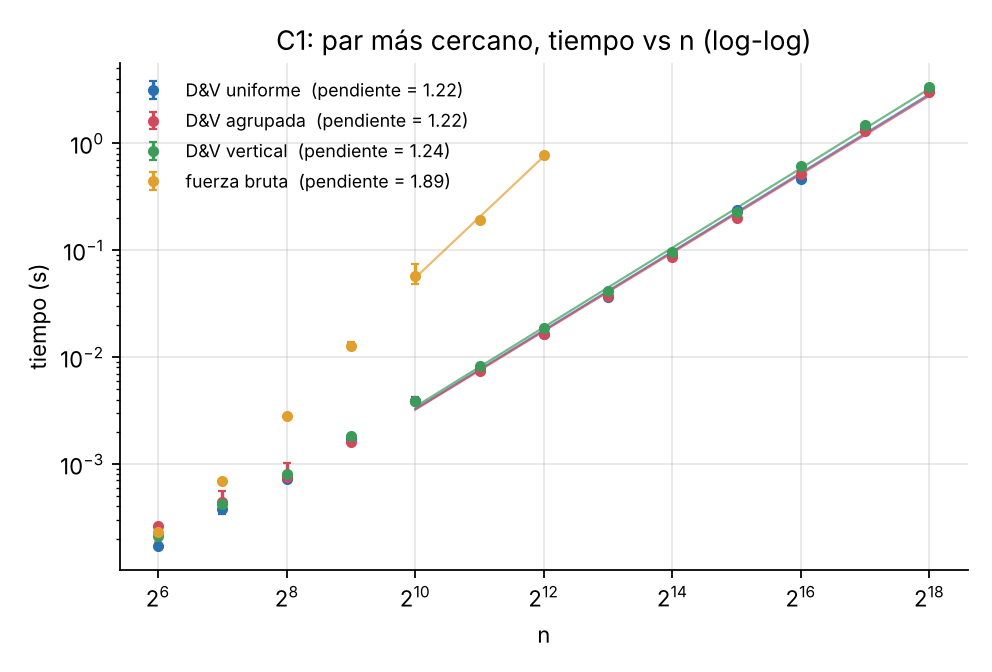
\includegraphics[width=0.49\linewidth]{figuras/c1_loglog.png}\hfill
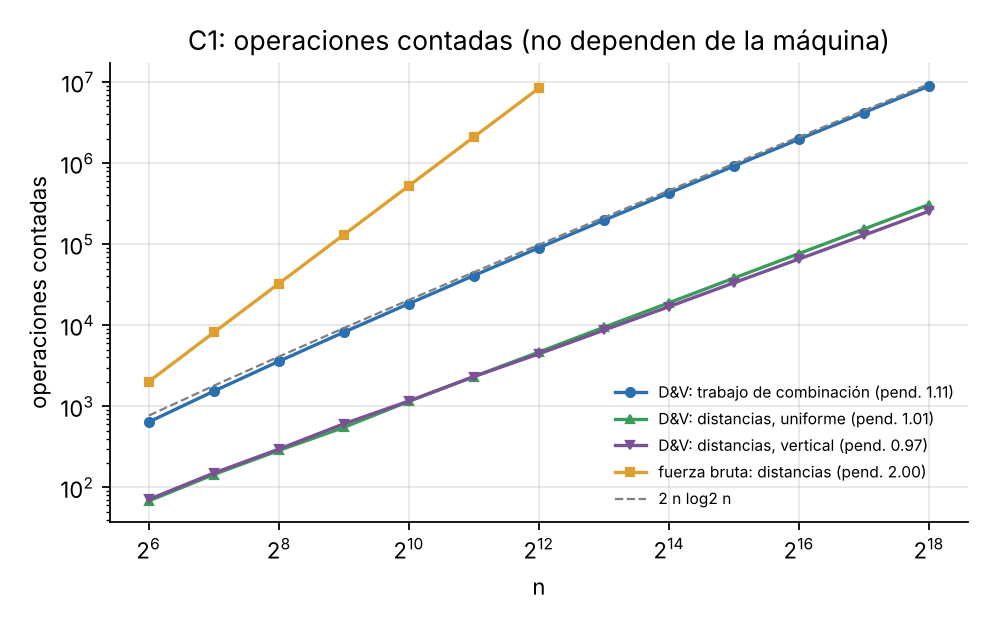
\includegraphics[width=0.49\linewidth]{figuras/c1_operaciones.png}
\caption{C1. Izquierda: tiempo (ajuste en $n\ge2^{10}$). Derecha: operaciones contadas.}
\end{figure}

\textbf{Resultado.} Pendientes de tiempo $\cUnoPendUni$ (uniforme), $\cUnoPendAgr$ (agrupada) y
$\cUnoPendVer$ (vertical); en $2^{10}..2^{14}$ están entre $\cUnoBajoMin$ y $\cUnoBajoMax$, cerca de la
referencia $\cUnoPendTeo$, y en $2^{14}..2^{18}$ suben a $\cUnoAltoMin$--$\cUnoAltoMax$ (caché, ver
sección~\ref{sec:discusion}). El trabajo de combinación \emph{contado} tiene pendiente $\cUnoPendComb$ y
la razón combinación$/(n\log_2 n)$ pasa de $\cUnoCombIni$ a $\cUnoCombFin$ (tiende a 2): coincide con la
teoría. Fuerza bruta: pendiente $\cUnoPendFB$ en tiempo y 2,00 contando distancias (son exactamente $\binom n2$); D\&V es más rápido desde $n=\cUnoCruce$ y $\cUnoSpeedup$
veces más rápido en $n=4096$. Máximo de vecinos revisados en la franja: $\cUnoMaxVecinos$ (cota 7).

% ------------------------------------------------------------- C2
\subsection{C2 -- Mapa de vóxeles}
\textbf{Hipótesis}: banco $\ge0$ y $C(n)\le3n$; $n$ inserciones en $\Th(n)$; la tabla ocupa $\Th(N)$ con
$N=\Th((L/r)^2)$ y la rejilla $\Th((L/r)^3)$.

\begin{figure}[H]
\centering
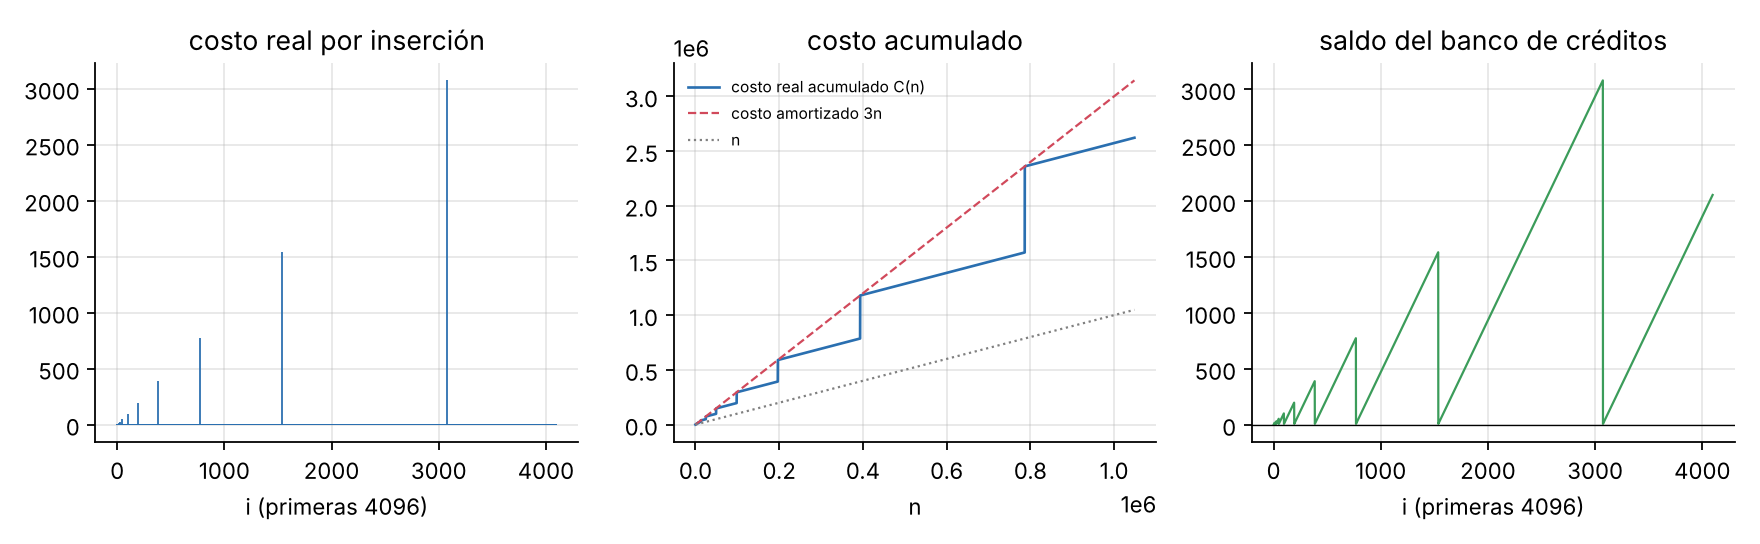
\includegraphics[width=0.94\linewidth]{figuras/c2_metodo_contable.png}\\[1mm]
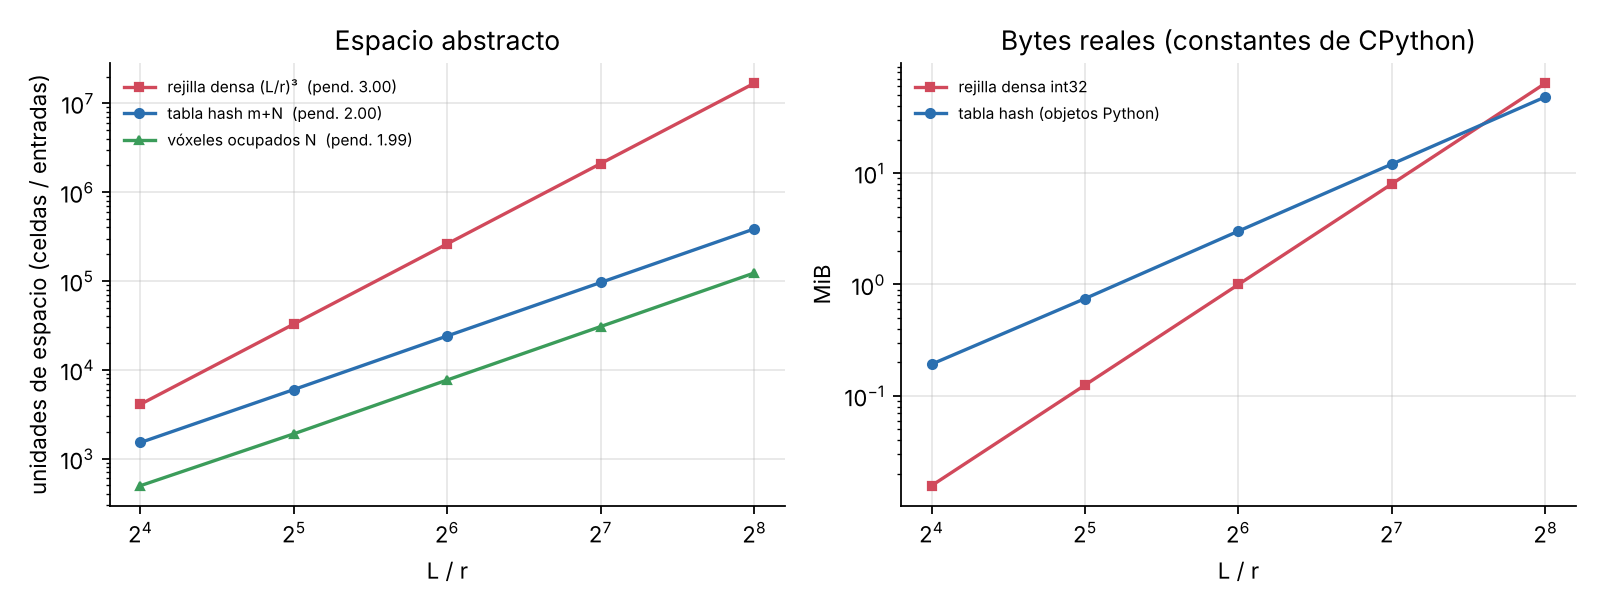
\includegraphics[width=0.80\linewidth]{figuras/c2_espacio.png}
\caption{C2. Arriba: método contable con $n=2^{20}$ (picos en cada duplicación, $C(n)\le3n$, banco $\ge0$).
Abajo: espacio para $L=64$\,m y $r$ de 4\,m a 0,25\,m.}
\end{figure}

\textbf{Resultado.} Con $n=\cDosN$: $C(n)=\cDosCosto\le3n=\cDosCota$, $\max C(n)/n=\cDosMaxRazon$, banco
mínimo $\cDosBancoMin\ge0$ y $\cDosDuplic$ duplicaciones: $C(n)/n$ oscila en diente de sierra entre
$\approx2$ y 3, como predice el análisis. Tiempo: pendiente $\cDosPendBajo$ mientras la tabla cabe en
caché y $\cDosPendAlto$ después ($\cDosUsIni$ a $\cDosUsFin\,\mu$s por inserción). Espacio frente a $L/r$:
vóxeles ocupados $\cDosPendN$, tabla $\cDosPendTabla$, rejilla $\cDosPendDensa$. En bytes, cada vóxel cuesta
$\approx\cDosBytesVox$\,B en CPython frente a 4\,B por celda \texttt{int32}: la tabla solo es más pequeña
desde $L/r=\cDosLrMax$ ($\cDosMiBTabla$ frente a $\cDosMiBDensa$\,MiB).

% ------------------------------------------------------------- C3
\subsection{C3 -- Cobertura mínima}
\textbf{Hipótesis}: el voraz es óptimo (frente a fuerza bruta) y detecta la infactibilidad; ``el más largo
primero'' no es óptimo; total $\Th(n\log n)$ y barrido $\Th(n)$.

\begin{figure}[H]
\centering
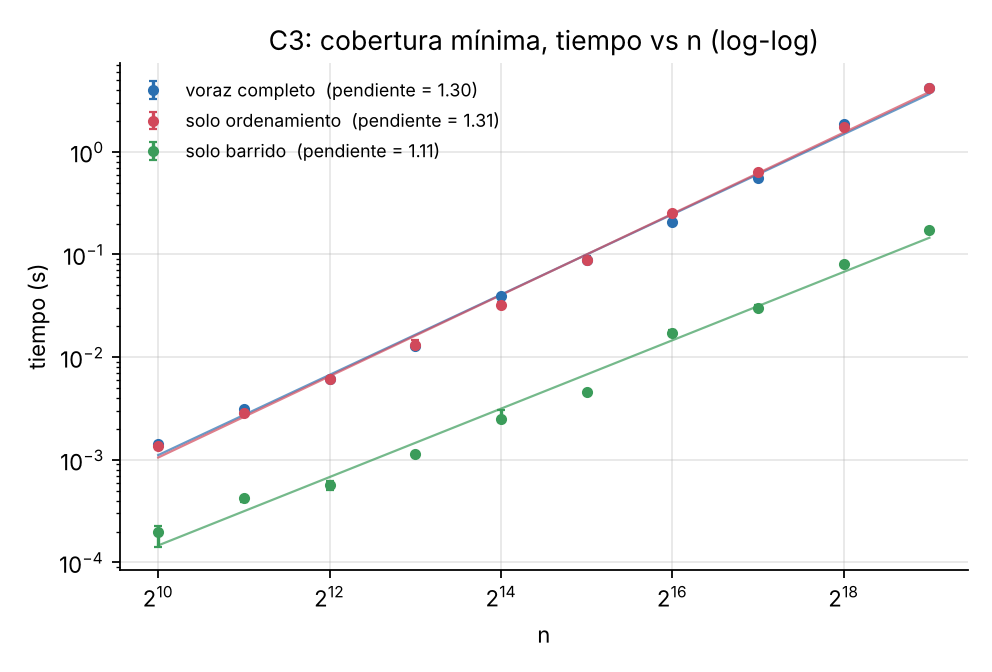
\includegraphics[width=0.49\linewidth]{figuras/c3_loglog.png}\hfill
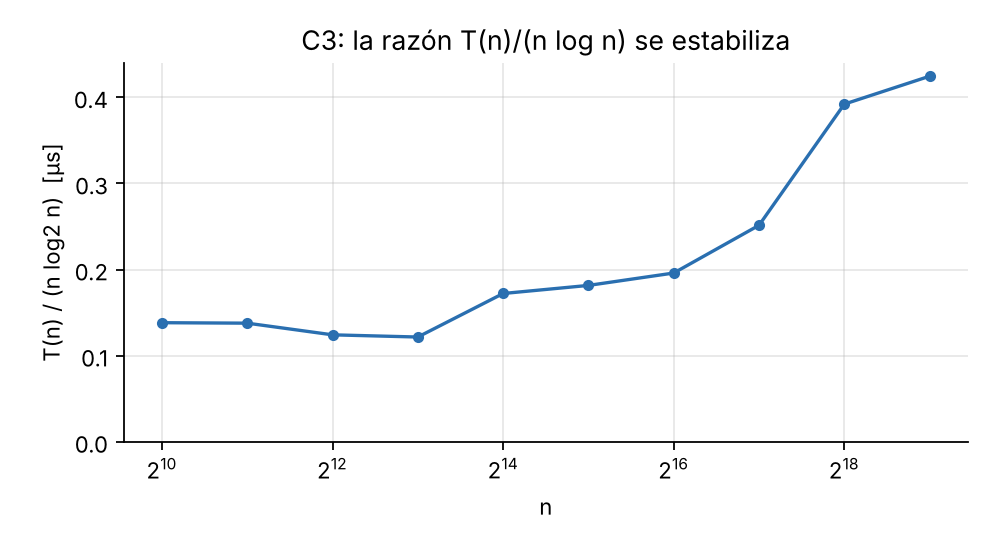
\includegraphics[width=0.49\linewidth]{figuras/c3_razon_nlogn.png}
\caption{C3. Izquierda: tiempo total, del ordenamiento y del barrido. Derecha: $T(n)/(n\log_2 n)$.}
\end{figure}

\textbf{Resultado.} En $\cTresInst$ instancias aleatorias con $n=4..11$: voraz igual al óptimo en
\textbf{$\cTresIguales$ de $\cTresFact$} factibles y $\cTresInfactOk$ de $\cTresInfact$ infactibles detectadas;
``el más largo primero'' fue subóptimo en $\cTresLargo$ casos (peor: $\cTresEjLargo$ tramos frente a
$\cTresEjOpt$). Pendiente total $\cTresPendTotalBajo$ en $2^{10}..2^{14}$ (referencia $\cTresPendTeo$) y
$\cTresPendTotal$ en todo el rango; las comparaciones contadas del merge sort tienen pendiente
$\cTresPendComp$. El barrido es solo el $\approx\cTresFracBarrido$\,\% del tiempo total (el resto es
ordenar) y tiene pendiente $\cTresPendBarridoBajo$ en $2^{10}..2^{14}$.

% ------------------------------------------------------------- C4
\subsection{C4 -- Backtracking en cuadrícula}\label{sec:val4}
\textbf{Hipótesis}: sin poda los nodos crecen exponencialmente con las celdas; la poda de Manhattan
devuelve la misma longitud con órdenes de magnitud menos nodos; BFS es $\Th(V)$; la poda no elimina el
crecimiento exponencial en cuadrículas grandes. 10 cuadrículas por tamaño, densidad de obstáculos $0{,}2$.

\begin{figure}[H]
\centering
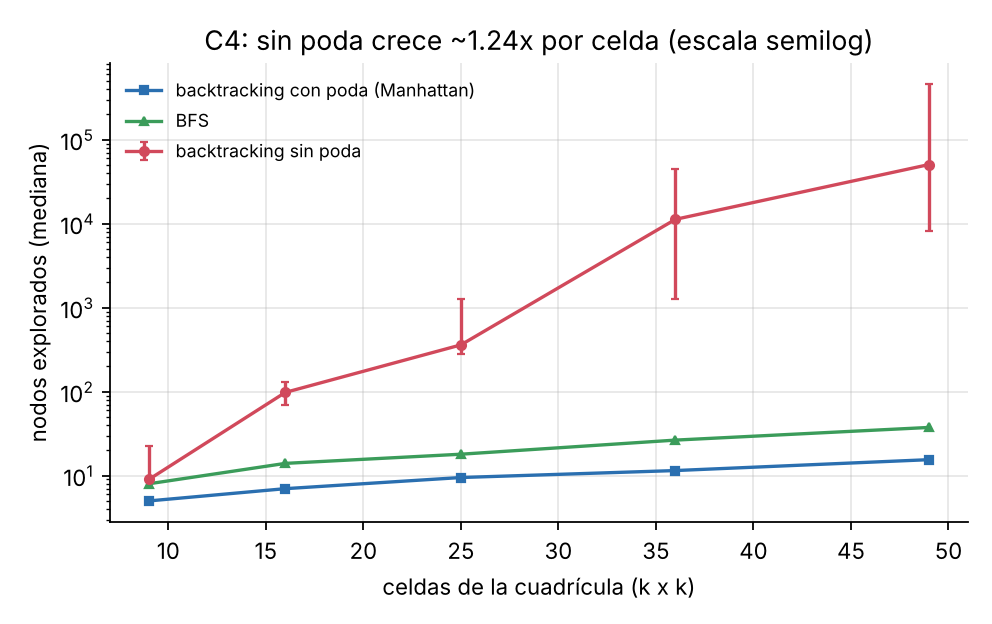
\includegraphics[width=0.49\linewidth]{figuras/c4_nodos_pequenas.png}\hfill
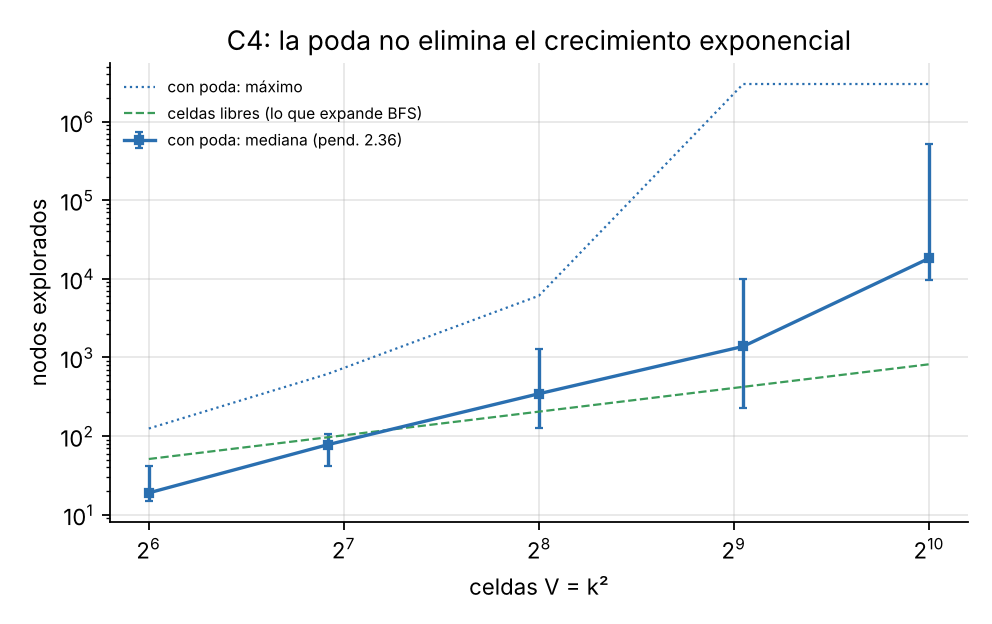
\includegraphics[width=0.49\linewidth]{figuras/c4_poda_escala.png}
\caption{C4. Izquierda: nodos explorados en cuadrículas pequeñas (escala semilogarítmica). Derecha:
nodos con poda al crecer la cuadrícula, frente a las celdas que expande BFS.}
\end{figure}

\begin{table}[H]
\centering\small
\caption{C4: nodos explorados (mediana de 10 cuadrículas). Los tres algoritmos dieron siempre la misma
longitud mínima. $^{*}$: alguna instancia superó el límite de $3\cdot10^6$ nodos.}
\begin{tabular}{lrrrrr}
\toprule
Cuadrícula & Celdas & Sin poda & Con poda & BFS & Sin poda / con poda \\
\midrule
\filas{tabla_c4.tex}
\bottomrule
\end{tabular}
\end{table}

\textbf{Resultado.} Sin poda los nodos se multiplican por $\approx\cCuatroFactor$ por cada celda (recta en
semilog): en $\cCuatroK\times\cCuatroK$ la mediana es $\cCuatroSinMed$ nodos ($\cCuatroTSin$\,s) frente a
$\cCuatroConMed$ con poda ($\cCuatroTCon$\,ms). BFS: pendiente de tiempo $\cCuatroPendBfs$ entre $2^{10}$
y $2^{20}$ celdas. Con poda, en cuadrículas mayores los nodos crecen con pendiente $\cCuatroPendPoda$
frente a 1 de BFS; en $\cCuatroPodaK\times\cCuatroPodaK$ la mediana es $\cCuatroPodaMed$ y el máximo
$\cCuatroPodaMax$ nodos ($\cCuatroPodaCortes$ de 10 cuadrículas alcanzaron el límite de $3\cdot10^6$): la
cota de Manhattan es floja cuando los obstáculos obligan a desvíos. En el
parqueadero (Anexo~\ref{anexo:extra}) la maniobra mide $\cCuatroParqLong$ movimientos: $\cCuatroParqSin$
nodos sin poda, $\cCuatroParqCon$ con poda y $\cCuatroParqBfs$ con BFS.

% ------------------------------------------------------------- C5
\subsection{C5 -- Árbol B+ en disco: E/S predichas frente a contadas}
\textbf{Hipótesis}: las fórmulas de la sección 3.5 predicen exactamente las E/S de la carga y de la búsqueda
puntual, y acotan las de los rangos. Bloques de 4\,096 bytes ($B=170$, $F=341$), $M=N/20$.

\begin{table}[H]
\centering\small
\caption{C5: construcción y búsqueda puntual (contado / predicho). Lecturas puntuales: máximo de 200 consultas.}
\label{tab:c5}
\begin{tabular}{rrccccr}
\toprule
$N$ & $M/B$ & $h$ & Lecturas carga & Escrituras carga & Lect. punto & Tiempo (s) \\
\midrule
\filas{tabla_c5_construccion.tex}
\bottomrule
\end{tabular}
\end{table}

\begin{figure}[H]
\centering
\begin{minipage}{0.52\linewidth}
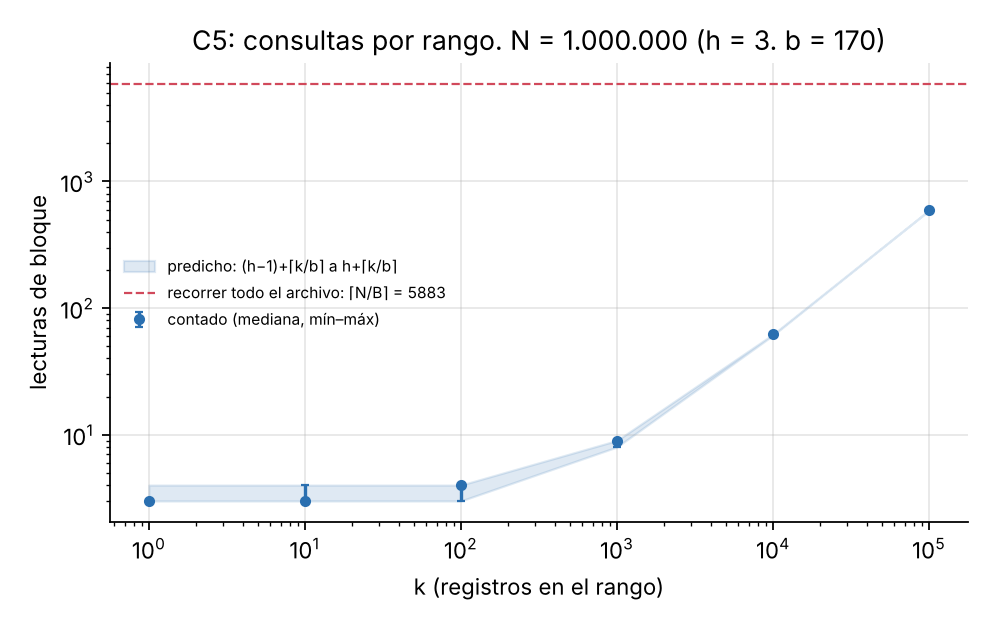
\includegraphics[width=\linewidth]{figuras/c5_rangos.png}
\end{minipage}\hfill
\begin{minipage}{0.45\linewidth}
\footnotesize\setlength{\tabcolsep}{3.5pt}
\captionof{table}{C5: lecturas por rango, $N=\cCincoNMax$ (50 consultas por $k$).}
\begin{tabular}{rrrrcc}
\toprule
$k$ & mín & med. & máx & predicho & ok \\
\midrule
\filas{tabla_c5_rangos.tex}
\bottomrule
\end{tabular}
\end{minipage}
\end{figure}

\textbf{Resultado.} En los 6 tamaños, las lecturas y escrituras de la carga masiva coinciden
exactamente con las predichas y la búsqueda puntual cuesta exactamente $h$ lecturas (Tabla~\ref{tab:c5});
las 300 consultas por rango quedaron dentro de la fórmula. Con $N=\cCincoNMax$ un rango pequeño
cuesta $\cCincoH$ lecturas frente a $\cCincoRecorrido$ de recorrer el archivo. E/S de la carga frente a $N$:
pendiente $\cCincoPendES$; tiempo: $\cCincoPendT$. Inserción de registros tardíos
($N=100\,000$): siempre $h$ lecturas; con hojas llenas (llenado 100\,\%) el $\cCincoInsCienDiv$\,\% de las
inserciones dividió una hoja ($\cCincoInsCienEscr$ escrituras en promedio) y con llenado 70\,\% el
$\cCincoInsSetentaDiv$\,\% ($\cCincoInsSetentaEscr$); la fórmula $1+2s+[\text{raíz}]$ se cumplió en las
$\cCincoInsCienExactas+\cCincoInsSetentaExactas$ inserciones. El efecto del tamaño de bloque está en el
Anexo~\ref{anexo:extra}.

% ------------------------------------------------------------- C6
\subsection{C6 -- 2-aproximación de cobertura de vértices}
\textbf{Hipótesis}: $|M|\le OPT\le|C|\le2\,OPT$ en el 100\,\% de los grafos; razón 2 exacta en el caso
ajustado; tiempo $\Th(V+E)$; fuerza bruta exponencial.

\begin{figure}[H]
\centering
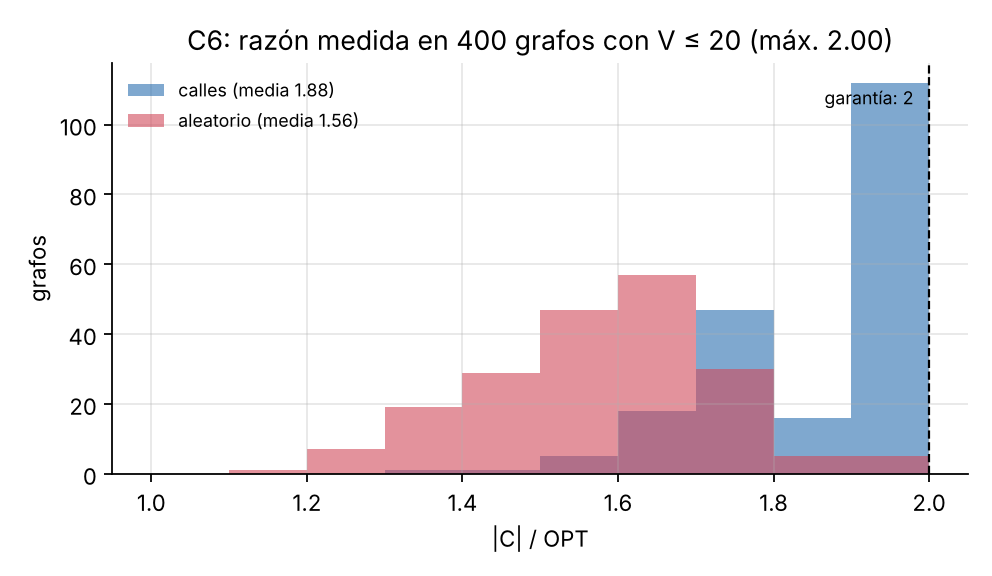
\includegraphics[width=0.49\linewidth]{figuras/c6_razones.png}\hfill
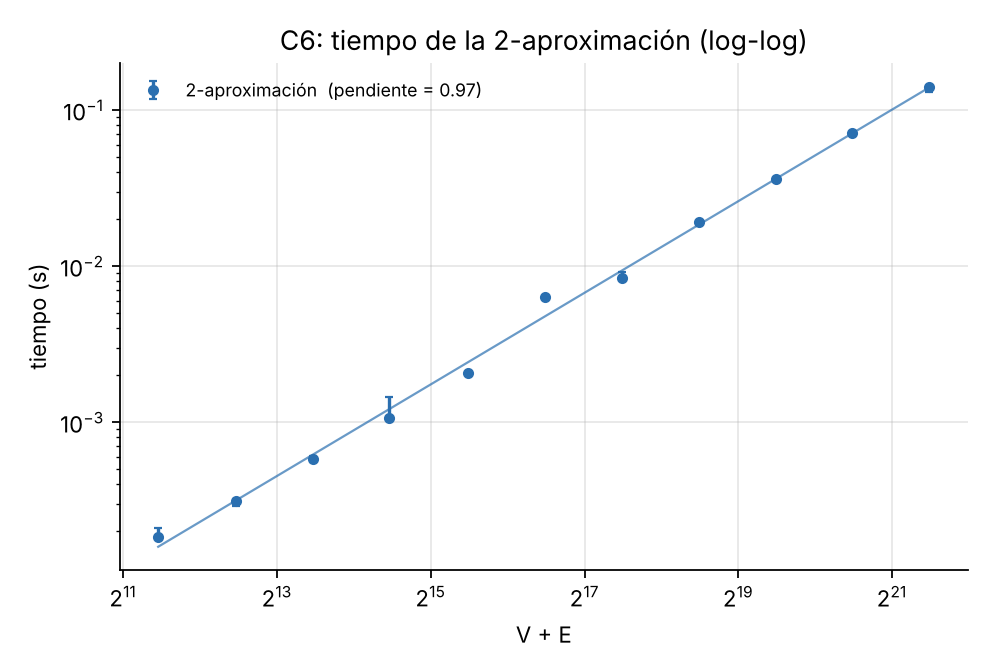
\includegraphics[width=0.49\linewidth]{figuras/c6_loglog.png}
\caption{C6. Izquierda: razón $|C|/OPT$ frente al óptimo por fuerza bruta. Derecha: tiempo frente a $V+E$.}
\end{figure}

\textbf{Resultado.} En $\cSeisGrafos$ grafos con $V\le20$ (redes de calles y $G(n,0{,}25)$) la desigualdad
$|M|\le OPT\le|C|\le2\,OPT$ se cumplió en $\cSeisCumplen$; razón media $\cSeisMediaCalles$ en calles y
$\cSeisMediaAleat$ en grafos aleatorios, entre $\cSeisMin$ y $\cSeisMax$. Caso ajustado: $|C|=\cSeisAjC$ y
$OPT=\cSeisAjOpt$, razón exactamente 2. Tiempo: pendiente $\cSeisPendT$ hasta $V+E\approx3\cdot10^6$.
La fuerza bruta multiplica su tiempo por $\approx\cSeisFactorFB$ por vértice ($\cSeisFBTmax$\,s con
$V=\cSeisFBVmax$). La heurística ``mayor grado primero'' dio en promedio una razón de $\cSeisGradoMax$
en estos grafos, mejor en la práctica, pero sin garantía: en el peor caso es $\Th(\log n)$ veces el óptimo.
% ------------------------------------------------------------- 5. DISCUSIÓN
\section{Discusión}\label{sec:discusion}

\textbf{Dónde coinciden teoría y práctica.} Todo lo que se puede contar coincide: $\binom n2$ distancias de
la fuerza bruta (C1), trabajo de combinación y comparaciones del merge sort con la pendiente de
$n\log_2 n$ (C1, C3), $C(n)\le3n$ con banco $\ge0$ (C2), optimalidad del voraz en el 100\,\% de los casos
(C3), igual longitud mínima en los tres algoritmos de C4, E/S de carga y búsqueda puntual exactas y rangos
dentro de la fórmula (C5), y razón $\le2$ en todos los grafos (C6).

\textbf{Dónde no coinciden y por qué.}
\begin{enumerate}
  \item \textbf{Caché y memoria.} Las pendientes de tiempo suben cuando $n>2^{14}$ (C1 hasta
  $\cUnoAltoMax$, C2 $\cDosPendAlto$, C3 $\cTresPendTotal$). En CPython cada punto o entrada es un objeto
  de $\approx100$\,B disperso en memoria; pasados los 4\,MiB de caché L2 cada acceso es más lento. El
  modelo RAM supone acceso uniforme; el modelo de memoria externa de C5, en cambio, cuenta justamente
  las transferencias, y por eso allí la predicción es exacta.
  \item \textbf{La pendiente de $n\log n$ no es 1} sino $\approx1{,}1$ en nuestros rangos.
  \item \textbf{Constantes del intérprete.} $\approx0{,}3\,\mu$s por unidad de $n\log n$ en C1, y
  $\approx\cDosBytesVox$\,B por vóxel en C2: la ventaja asintótica de la tabla hash solo se ve en bytes
  desde $L/r=\cDosLrMax$.
  \item \textbf{Cotas de peor caso que no se alcanzan.} El lema de los 7 dio como máximo
  $\cUnoMaxVecinos$; la poda de C4 es muy buena en cuadrículas pequeñas, pero en las grandes la distancia
  de Manhattan subestima los desvíos y el árbol vuelve a crecer muy rápido: la cota del peor caso sigue
  siendo exponencial y BFS es la opción correcta para caminos sin restricciones. En C6 la razón promedio
  ($\cSeisMediaCalles$ y $\cSeisMediaAleat$) está por debajo de 2, que es una garantía de peor caso.
\end{enumerate}
La máquina es virtual y compartida (2 núcleos, Intel Xeon 2,1\,GHz, CPython 3.13); por eso usamos la
mediana de 5 repeticiones y contamos operaciones además del tiempo.

% ------------------------------------------------------------- 6. CONCLUSIONES
\section{Conclusiones y reparto del trabajo}

Los seis componentes funcionan, tienen pruebas (44, todas aprobadas) y cada afirmación de complejidad
está respaldada por una prueba y por un experimento. Lo más claro del proyecto: (i) en C1 y C3 el término
$n\log n$ lo pone la mezcla/ordenamiento, no las distancias ni el barrido; (ii) el método contable de C2
explica por qué duplicar la tabla cuesta $O(1)$ amortizado aunque una inserción cueste $\Th(N)$; (iii) en
C4 la poda reduce los nodos en órdenes de magnitud pero no cambia el peor caso; (iv) en C5 contar
bloques permite predecir el costo exacto, cosa que el tiempo no logra; (v) en C6 una prueba de dos líneas
garantiza la razón 2 frente a un problema NP-difícil.

\begin{table}[H]
\centering\small
\begin{tabular}{ll}
\toprule
Integrante & Componentes a cargo \\
\midrule
Santiago Felipe Fajardo & C1 (par más cercano) y C2 (tabla hash de vóxeles) \\
Sebastián Páez Castañeda & C3 (cobertura voraz) y C4 (backtracking) \\
Johan Sebastián Acuña & C5 (árbol B+ en disco) y C6 (cobertura de vértices) \\
Todos & experimentos, informe y diapositivas \\
\bottomrule
\end{tabular}
\end{table}

\textbf{Herramientas.} Los algoritmos de C1 a C6 los implementó el equipo; \texttt{sorted}
y \texttt{dict} solo aparecen en pruebas y experimentos como referencia, y NumPy solo para generar datos y
ajustar pendientes. El uso de asistentes de IA se declara en el \texttt{README.md}.

% ------------------------------------------------------------- REFERENCIAS
\section*{Referencias}
\addcontentsline{toc}{section}{Referencias}
\begin{enumerate}[label={[\arabic*]},leftmargin=*,itemsep=0pt]
\footnotesize
\item T. H. Cormen, C. E. Leiserson, R. L. Rivest y C. Stein. \emph{Introduction to Algorithms}, 4.ª ed. MIT Press, 2022.
\item J. Kleinberg y É. Tardos. \emph{Algorithm Design}. Pearson, 2006.
\item M. I. Shamos y D. Hoey. Closest-point problems. \emph{16th IEEE Symp. on Foundations of Computer Science}, 151--162, 1975.
\item M. Ben-Or. Lower bounds for algebraic computation trees. \emph{Proc. 15th ACM STOC}, 80--86, 1983.
\item M. Teschner et al. Optimized spatial hashing for collision detection of deformable objects. \emph{Vision, Modeling, and Visualization}, 2003.
\item M. Bousquet-Mélou, A. J. Guttmann e I. Jensen. Self-avoiding walks crossing a square. \emph{J. Physics A}, 38(42):9159--9181, 2005.
\item A. Aggarwal y J. S. Vitter. The input/output complexity of sorting and related problems. \emph{Comm. ACM}, 31(9):1116--1127, 1988.
\item R. Bayer y E. McCreight. Organization and maintenance of large ordered indexes. \emph{Acta Informatica}, 1:173--189, 1972.
\item R. M. Karp. Reducibility among combinatorial problems. En \emph{Complexity of Computer Computations}, 85--103, 1972.
\item S. Khot y O. Regev. Vertex cover might be hard to approximate to within $2-\varepsilon$. \emph{J. Comput. Syst. Sci.}, 74(3):335--349, 2008.
\end{enumerate}
% ------------------------------------------------------------- ANEXOS
\clearpage
\appendix

\section{Plan de experimentos con hipótesis}\label{anexo:plan}

\begin{table}[H]
\centering\small
\begin{tabularx}{\linewidth}{>{\bfseries}p{1.1cm} X >{\raggedright\arraybackslash}p{2.9cm} >{\raggedright\arraybackslash}p{3.15cm}}
\toprule
Comp. & Hipótesis & Tamaños & Criterio de aceptación \\
\midrule
C1 & D\&V $\Th(n\log n)$ en 3 distribuciones; fuerza bruta $\Th(n^2)$; $\le7$ vecinos en la franja;
trabajo de combinación $\approx2n\log_2 n$ & $2^6..2^{18}$ (FB $2^6..2^{12}$) & pendiente $\approx1{,}1$ y
$T/(n\log n)$ acotada; FB $\approx2$ \\
C2 & banco $\ge0$ y $C(n)\le3n$; $n$ inserciones $\Th(n)$; $N=\Th((L/r)^2)$, tabla $\Th(N)$, rejilla
$\Th((L/r)^3)$ & $2^{10}..2^{20}$; $L/r=16..256$ & $\max C(n)/n\le3$; pendientes $\approx1$, 2, 3 \\
C3 & voraz $=$ óptimo; ``más largo primero'' no óptimo; total $\Th(n\log n)$, barrido $\Th(n)$ &
2000 instancias $n\le11$; $2^{10}..2^{19}$ & 100\,\% de coincidencias \\
C4 & sin poda exponencial; poda: misma longitud y muchos menos nodos; BFS $\Th(V)$; la poda no elimina
el peor caso & $k=3..7$ (10 cuadrículas c/u); BFS $2^{10}..2^{20}$ celdas & razón sin/con creciente;
BFS pendiente $\approx1$ \\
C5 & carga: $1+\lceil N/B\rceil$ lecturas y $L+\sum I_j+1$ escrituras; punto: $h$; rango:
$[h-1,h]+\lceil k/b\rceil$; inserción $h$ lecturas y $1+2s+[\text{raíz}]$ escrituras &
$N=10^5..10^6$ ($\times1{,}58$), $M=N/20$; $k=1..10^5$; bloques 512--8192\,B & contado $=$ predicho
(o dentro de la cota) en el 100\,\% \\
C6 & $|M|\le OPT\le|C|\le2\,OPT$; razón 2 en el caso ajustado; $\Th(V+E)$; fuerza bruta exponencial &
400 grafos con $V\le20$; $V=2^{10}..2^{20}$ & 100\,\% dentro de la cota; pendiente $\approx1$ \\
\bottomrule
\end{tabularx}
\end{table}

\section{Resultados adicionales}\label{anexo:extra}

\begin{figure}[H]
\centering
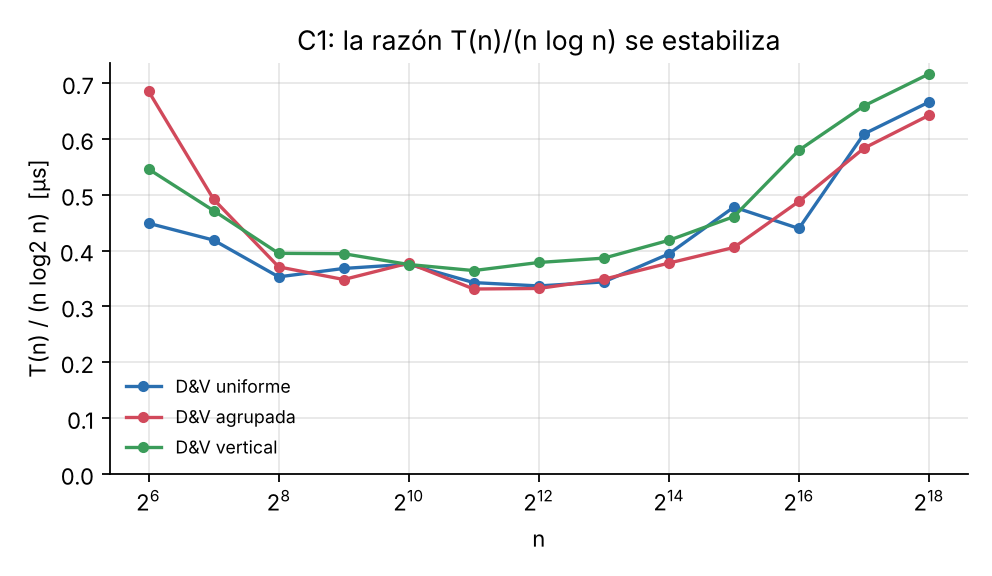
\includegraphics[width=0.48\linewidth]{figuras/c1_razon_nlogn.png}\hfill
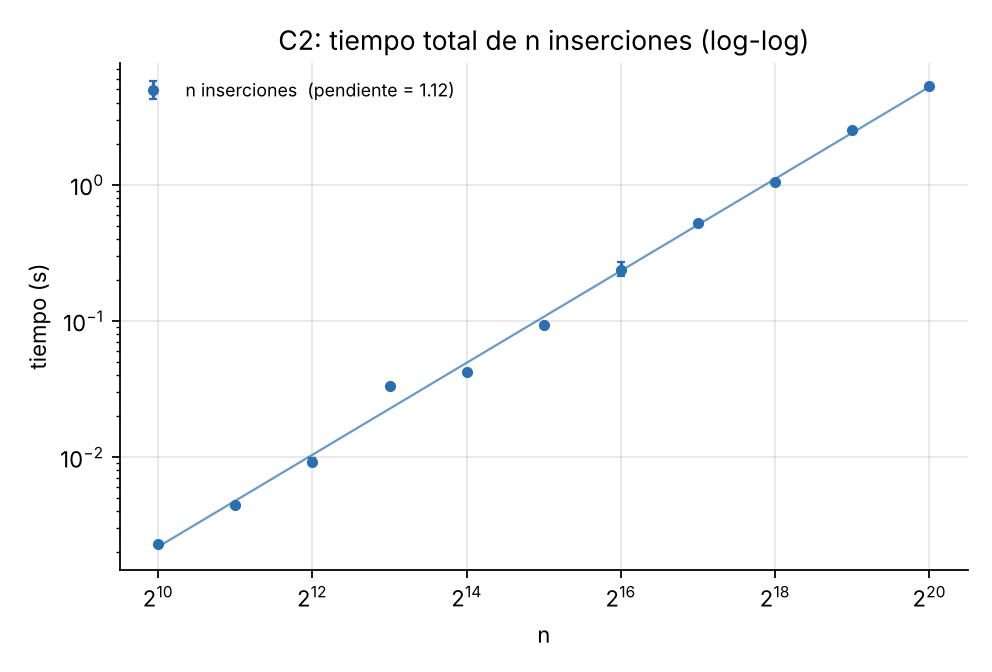
\includegraphics[width=0.48\linewidth]{figuras/c2_loglog.png}\\[1mm]
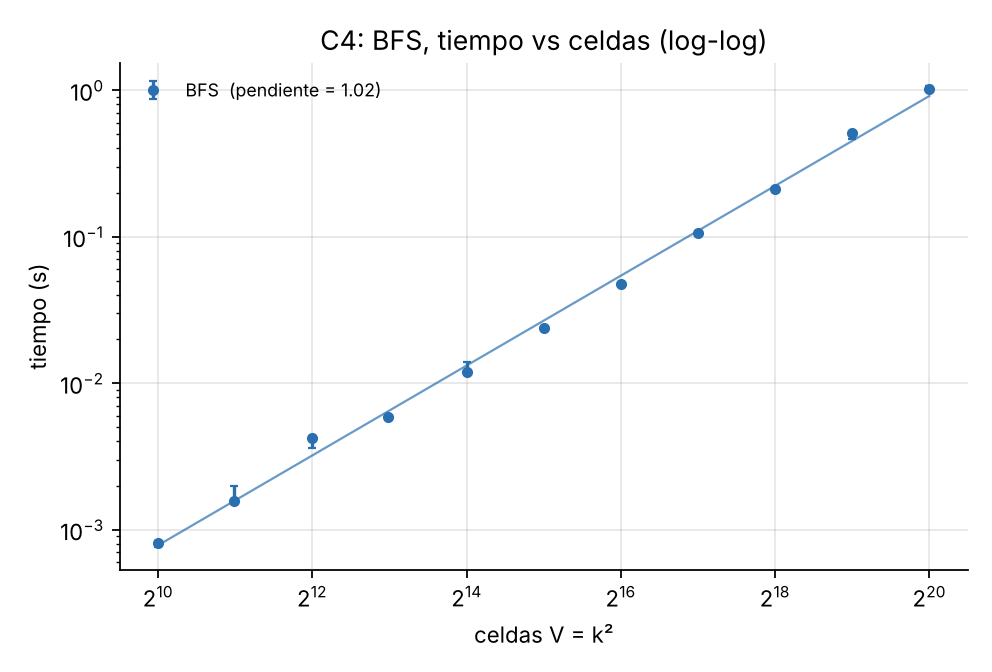
\includegraphics[width=0.48\linewidth]{figuras/c4_bfs_loglog.png}\hfill
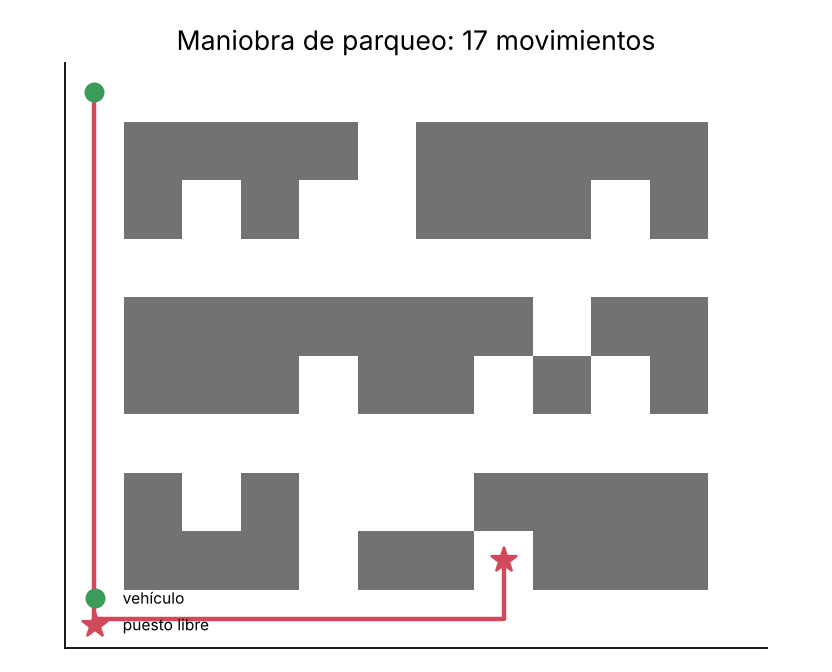
\includegraphics[width=0.40\linewidth]{figuras/c4_parqueadero.png}\\[1mm]
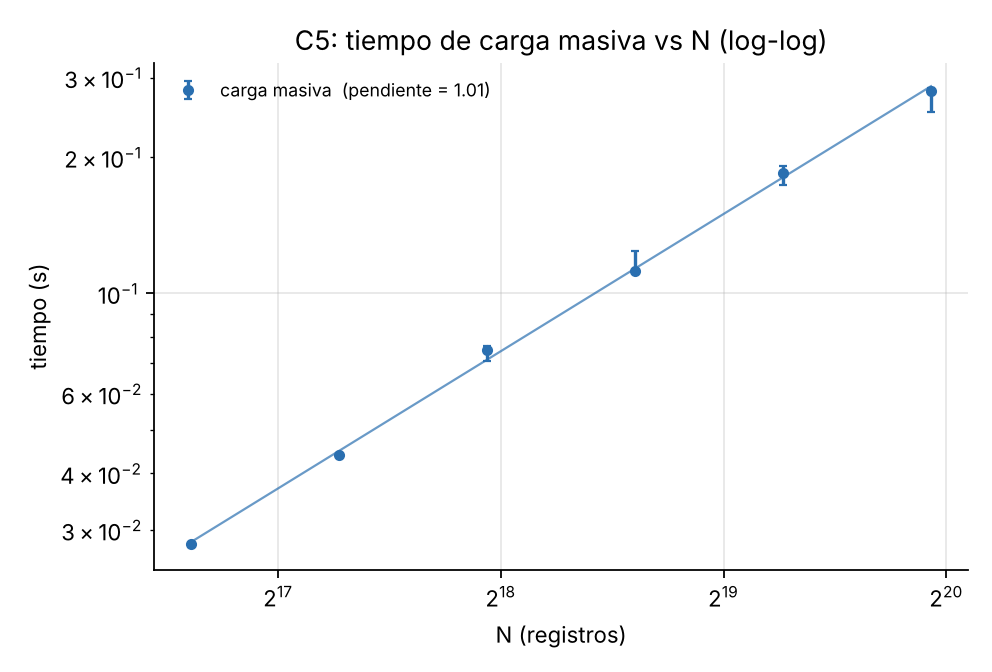
\includegraphics[width=0.48\linewidth]{figuras/c5_carga_loglog.png}
\caption{C1: $T(n)/(n\log n)$. C2: tiempo de $n$ inserciones. C4: BFS hasta $2^{20}$ celdas y
maniobra de parqueo encontrada con poda. C5: tiempo de la carga masiva.}
\end{figure}

\begin{table}[H]
\centering\small
\caption{C5: efecto del tamaño de bloque con $N=\cCincoNMax$ (contado / predicho; rango de $k=10\,000$).}
\begin{tabular}{rrrcrrr}
\toprule
Bloque (B) & $b$ & $f$ & $h$ & Lect. punto & Lect. rango (med.) & Cota $h+\lceil k/b\rceil$ \\
\midrule
\filas{tabla_c5_bloque.tex}
\bottomrule
\end{tabular}
\end{table}

\section{Reproducibilidad}
Desde la raíz del repositorio: \texttt{pip install -r requirements.txt};
\texttt{python -m pytest -q} (44 pruebas); \texttt{python -m experimentos.ejecutar\_todos} (todos los CSV,
JSON y PNG de \texttt{resultados/}; \texttt{--rapido} para una versión corta);
\texttt{python informe/generar\_valores.py} (regenera las cifras de este informe). Semilla fija: 6.

\end{document}
